\documentclass[11pt]{article}
% \documentclass[11pt,twocolumn]{article}
\usepackage{times} % Times New Roman font
\usepackage{graphicx} % For figures
\usepackage{amsmath} % For mathematical expressions and symbols
\usepackage{booktabs} % For tables
\usepackage{hyperref} % For hyperlinks
\usepackage{geometry} % Custom margins
\usepackage{fancyhdr} % Custom headers and footers
\usepackage{xcolor}
\usepackage{subfiles}
\usepackage{multicol}
\usepackage{titlesec} % Add this line to your package imports
\usepackage{float}
\usepackage{algorithm}
\usepackage{algpseudocode}

% Adjust the space before and after sections
\titlespacing\section{0pt}{10pt}{10pt}

% Adjust the space before and after subsections
\titlespacing\subsection{0pt}{8pt}{8pt}

% Adjust the space before and after subsubsections
\titlespacing\subsubsection{0pt}{6pt}{6pt}

\setlength{\parindent}{0pt}

\geometry{
  top=1cm,
  bottom=1.5cm,
  left=1.75cm,
  right=1.75cm,
  headsep=0cm
  % includehead, % Include space for the header
  % includefoot, % Include space for the footer
  % headheight=1pt % Height of the header
}
\definecolor{grey}{gray}{0.5}
\fancypagestyle{plain}{
\fancyhead{}
\chead{\color{grey}\fontsize{8pt}{12pt}\selectfont \textbf{MECH0020\_AY2023-24}}
\fancyfoot[C]{\color{grey}\fontsize{10pt}{12pt}\selectfont \thepage}
\renewcommand{\headrulewidth}{0pt}
}

\pagestyle{plain}

% \title{\textbf{Title of the Paper}}
% \author{\textbf{Student Name and Number} \\
% \fontsize{12pt}{14pt}\selectfont Mechanical Engineering Department, University College London}
\title{\fontsize{16pt}{19pt}\selectfont\textbf{Title of the Paper}}
\author{\fontsize{14pt}{17pt}\selectfont\textbf{Student Name and Number} \\
\fontsize{12pt}{14pt}\selectfont Mechanical Engineering Department, University College London}
\date{} % No date to mimic the template

\begin{document}

\maketitle

\subfile{abstract.tex}


\setlength{\columnsep}{1.27cm}
\begin{multicols}{2}
\subfile{introduction.tex}

\subfile{literature_review.tex}

\subfile{theory_and_calculation.tex}

\subfile{result_and_discussion.tex}

% \section{Mathematical Expressions and Symbols}
% \label{sec:mathematical_expressions}
% Mathematical expressions and symbols should be inserted using the equation tool. For example, the Fourier series analysis can be represented as:
% \begin{equation}
% f(x)=a_0+\sum_{n=1}^{\infty}a_n\cos\left(\frac{n\pi x}{L}\right)+b_n\sin\left(\frac{n\pi x}{L}\right)
% \end{equation}

% \section{Results and Discussion}
% \label{sec:results_discussion}
% This section may each be divided by subheadings or may be combined. 

% \subsection{Preparation of Figures and Tables}
% \label{subsec:figures_tables}
% Embed all figures and tables at appropriate places within the text. For example, Figure~\ref{fig:example}.

% \begin{figure}[H]
% \centering
% 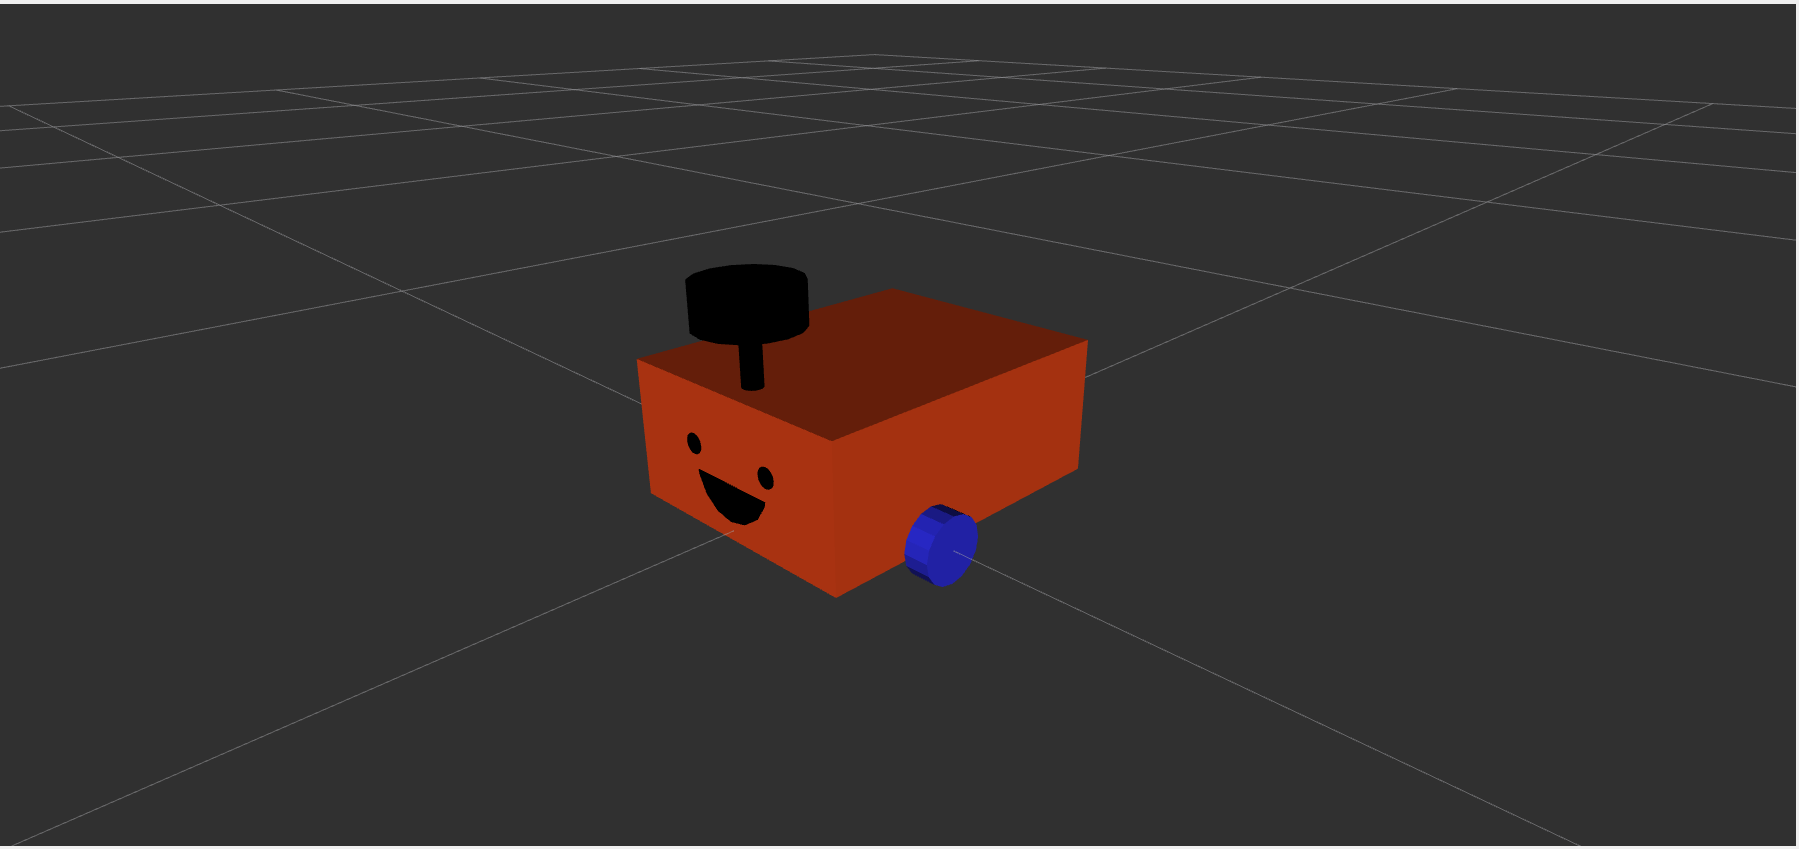
\includegraphics[width=0.8\linewidth]{figs/robot.png}
% \caption{Example figure caption.}
% \label{fig:example}
% \end{figure}

% \begin{table}[ht]
% \centering
% \caption{Example table caption.}
% \label{tab:example}
% \begin{tabular}{lcr}
% \toprule
% Column 1 & Column 2 & Column 3 \\
% \midrule
% Row 1 & Data & Data \\
% Row 2 & Data & Data \\
% \bottomrule
% \end{tabular}
% \end{table}

% \section{Conclusions}
% \label{sec:conclusions}
% Each report should contain a conclusion section within 250-450 words which may contain the major outcome of the work.

% % Acknowledgements section
% \section*{Acknowledgements}
% All acknowledgments (if any) should be included here.
\end{multicols}
% % References
% \begin{thebibliography}{99}
% \bibitem{b1} Author, "Title of the paper," \textit{Journal Name}, vol. xx, no. xx, pp. xxx-xxx, month, year.
% \bibitem{b2} Author, "Title of the paper," \textit{Journal Name}, vol. xx, no. xx, pp. xxx-xxx, month, year.
% \end{thebibliography}
\end{document}
